\documentclass[9pt,a4paper]{extarticle}

\usepackage[T1]{fontenc}
\usepackage[margin=1.75cm]{geometry}
\usepackage{booktabs}
\usepackage{graphicx}
\usepackage{amsmath}
\usepackage{siunitx}
\usepackage{enumitem}
\usepackage{microtype}
\usepackage[hidelinks]{hyperref}
\usepackage{caption}

\captionsetup{font=small,labelfont=bf,skip=4pt}
\setlength{\parskip}{2pt}
\setlist[itemize]{itemsep=2pt,topsep=3pt,leftmargin=1.3em}

\title{\vspace{-1.2cm}\textbf{Simulating Memory: Devices to Systems}\\[2pt]
\large Should the 2\,MB L2 cache in our accelerator be SRAM or STT-MRAM?}
\author{Jayadeep Koya \\
\small\texttt{\href{https://github.com/Jayadeep-4/AMCAS-assignment1}%
{github.com/Jayadeep-4/AMCAS-assignment1}}}
\date{\small ECE2.414 Advanced Memory Circuits and Systems \\
IIIT Hyderabad, Monsoon 2026}

\begin{document}
\maketitle
\vspace{-0.6cm}

\section{Tools and setup}

\begin{center}\small
\renewcommand{\arraystretch}{1.25}
\begin{tabular}{|c|l|l|l|}
\hline
\textbf{Part} & \textbf{Tool} & \textbf{Resolves} & \textbf{Produces} \\
\hline
A & ngspice 42 & 6T bitcell read margin & \SI{540.8}{mV} signal, \SI{434}{mV} trip point \\
\hline
B & CACTI 7 & SRAM array organisation & \SI{2.9018}{ns} hit latency, \SI{11.474}{mm^2} \\
\hline
C & NVSim & same array, MRAM bitcell & \SI{1.589}{ns} hit latency, \SI{3.590}{mm^2} \\
\hline
E & gem5 25.1.0.1 & whole program execution & IPC, miss rate, L2 miss trace \\
\hline
D & DRAMsim3 & DDR4 channel timing & row-buffer hit rate, read latency \\
\hline
\end{tabular}
\end{center}

Part~E takes its L2 hit latency from Parts~B and~C, and its capacity trade
from NVSim's areas. Part~D takes its trace from Part~E, so the two were
run in that order.

\paragraph{Assumptions.}
\begin{itemize}
\item All parts use 45\,nm. Part~A uses PTM bulk BSIM4 model cards and the
other parts use the shipped 45\,nm configurations.
\item gem5 runs at its default \SI{2}{GHz}, so \SI{2.9018}{ns} becomes 6
cycles and \SI{1.589}{ns} becomes 4 cycles.
\item Ratios between configurations are reported rather than absolute
values, because errors compound along the chain. Sec.~\ref{sec:err}
quantifies this.
\end{itemize}

\paragraph{DRAMsim3 in place of Ramulator.}
\begin{itemize}
\item The assignment specifies Ramulator 2.0, whose executable and YAML
interface no longer exists. Version 2.1 is a Python module with a
different trace format.
\item Tasks~1 and~2 reproduce in version 2.1 whereas Tasks~3 and~4 do not.
The address mapping and channel count settings had no effect, and every
configuration mapped the whole stream to one controller.
\item DRAMsim3 responds to both settings and accepts a per request arrival
cycle, so it replays the request spacing gem5 produced. Tasks~1 and~2 were
run in both simulators as a cross check.
\end{itemize}






\section{Part A - NgSpice}
\label{sec:a}

A 6T cell at 45\,nm with $Q=0$ and $\overline{Q}=1$ stored. Bitlines
precharge to $V_{DD}$ on \SI{180}{fF}, the wordline rises at
\SI{1.05}{ns}, and $\Delta V$ is measured at \SI{2.0}{ns}. The cell ratio
$W(\mathrm{MN1})/W(\mathrm{MA1})$ is $0.20/0.16 = 1.25$, below the 1.5
normally required for read stability.

A separate DC sweep gives the $q \rightarrow \overline{q}$ inverter trip
point as \SI{434}{mV} at \SI{1.1}{V} and \SI{282}{mV} at \SI{0.7}{V}. Read
disturb is judged against these.

\begin{table}[!ht]\centering\small
\caption{Read margin and read disturb. All rows use the specified
\SI{180}{fF} bitline except one. At that value the cell always recovers,
so a single run at \SI{400}{fF} is included to show the failure Task~2
expects. Trip point is \SI{434}{mV} at \SI{1.1}{V} and \SI{282}{mV} at
\SI{0.7}{V}.}
\label{tab:a}
\renewcommand{\arraystretch}{1.2}
\begin{tabular}{|c|c|c|c|r|r|r|}
\hline
$V_{DD}$ & $W_{acc}$ & $T$ & $C_{BL}$ & $\Delta V$ at 2\,ns & $q_{max}$ & $q$ at 3.9\,ns \\
 & (\si{\micro m}) & (\si{\celsius}) & (fF) & (mV) & (mV) & (mV) \\
\hline
\SI{1.1}{V} & 0.16 & 27 & 180 & 540.8 & 270.3 &  31.8 \\
\hline
\SI{1.1}{V} & 0.24 & 27 & 180 & 498.6 & 475.1 &  22.5 \\
\hline
\SI{1.1}{V} & 0.24 & 85 & 180 & 302.7 & 547.5 &  33.2 \\
\hline
\SI{1.1}{V} & 0.24 & 85 & 400 &  77.3 & 586.0 & 291.3 \\
\hline
\SI{1.1}{V} & 0.16 & 85 & 180 & 514.8 & 300.1 &  38.6 \\
\hline
\SI{0.7}{V} & 0.16 & 85 & 180 & 285.4 & 157.2 &  34.0 \\
\hline
\SI{0.7}{V} & 0.24 & 85 & 180 & 334.2 & 221.7 &  22.4 \\
\hline
\end{tabular}
\end{table}

\paragraph{Does the bitcell read correctly at \SI{0.7}{V} and
\SI{85}{\celsius}?}

Yes. $q_{max}$ is 56\,\% of the \SI{282}{mV} trip point at nominal sizing
and 79\,\% with the widened access devices, and $\Delta V$ is eleven times
the \SI{25}{mV} sense amplifier offset. The cell is in fact safer at
\SI{0.7}{V} than at \SI{1.1}{V}, where the \SI{0.24}{\micro m} variant
reaches 109\,\% of trip, because lowering $V_{DD}$ weakens the access
transistor faster than it weakens the latch.

\paragraph{Task 1.}

$\Delta V = v(\overline{BL}) - v(BL)$ at $t = \SI{2}{ns}$ is
\SI{540.8}{mV}, against the \SI{69}{mV} reference, a ratio of
$7.8\times$.

Most of that gap is the measurement instant. The wordline rises at
\SI{1.05}{ns}, so \SI{2}{ns} gives the bitline \SI{950}{ps} to discharge,
about ten times a realistic sense amplifier enable delay.

The rest is the mechanism. In a 6T read the bitline starts at full
$V_{DD}$ and the cell pulls it down with a roughly constant current, so
the signal grows with time. The reference figure comes from charge
sharing, which is fixed by a capacitance ratio and does not grow at all.
Comparing them at one instant is comparing a slope against a constant.

\paragraph{Task 2.}

$v(Q)$ does move during the read. At nominal sizing the stored \texttt{0}
rises to \SI{270}{mV}, well short of the trip point.

Widening the access devices to \SI{0.24}{\micro m} drops the cell ratio to
0.83 and pushes the peak to \SI{475}{mV}, above the \SI{434}{mV} trip
point. The cell still recovers, because the disturb lasts only as long as
the bitline is discharging. The wider device is also faster to sense but
worse if you wait, since once $Q$ rises the voltage across the discharge
path collapses and $\Delta V$ at \SI{2}{ns} actually falls.

Whether the cell recovers depends on the bitline. With bare \SI{180}{fF}
capacitors the bitlines discharge and the stress ends on its own. On a
\SI{400}{fF} bitline at \SI{85}{\celsius} the peak reaches \SI{586}{mV}
and $Q$ never returns to zero, so the read destroys the stored value.

\begin{figure}[!ht]\centering
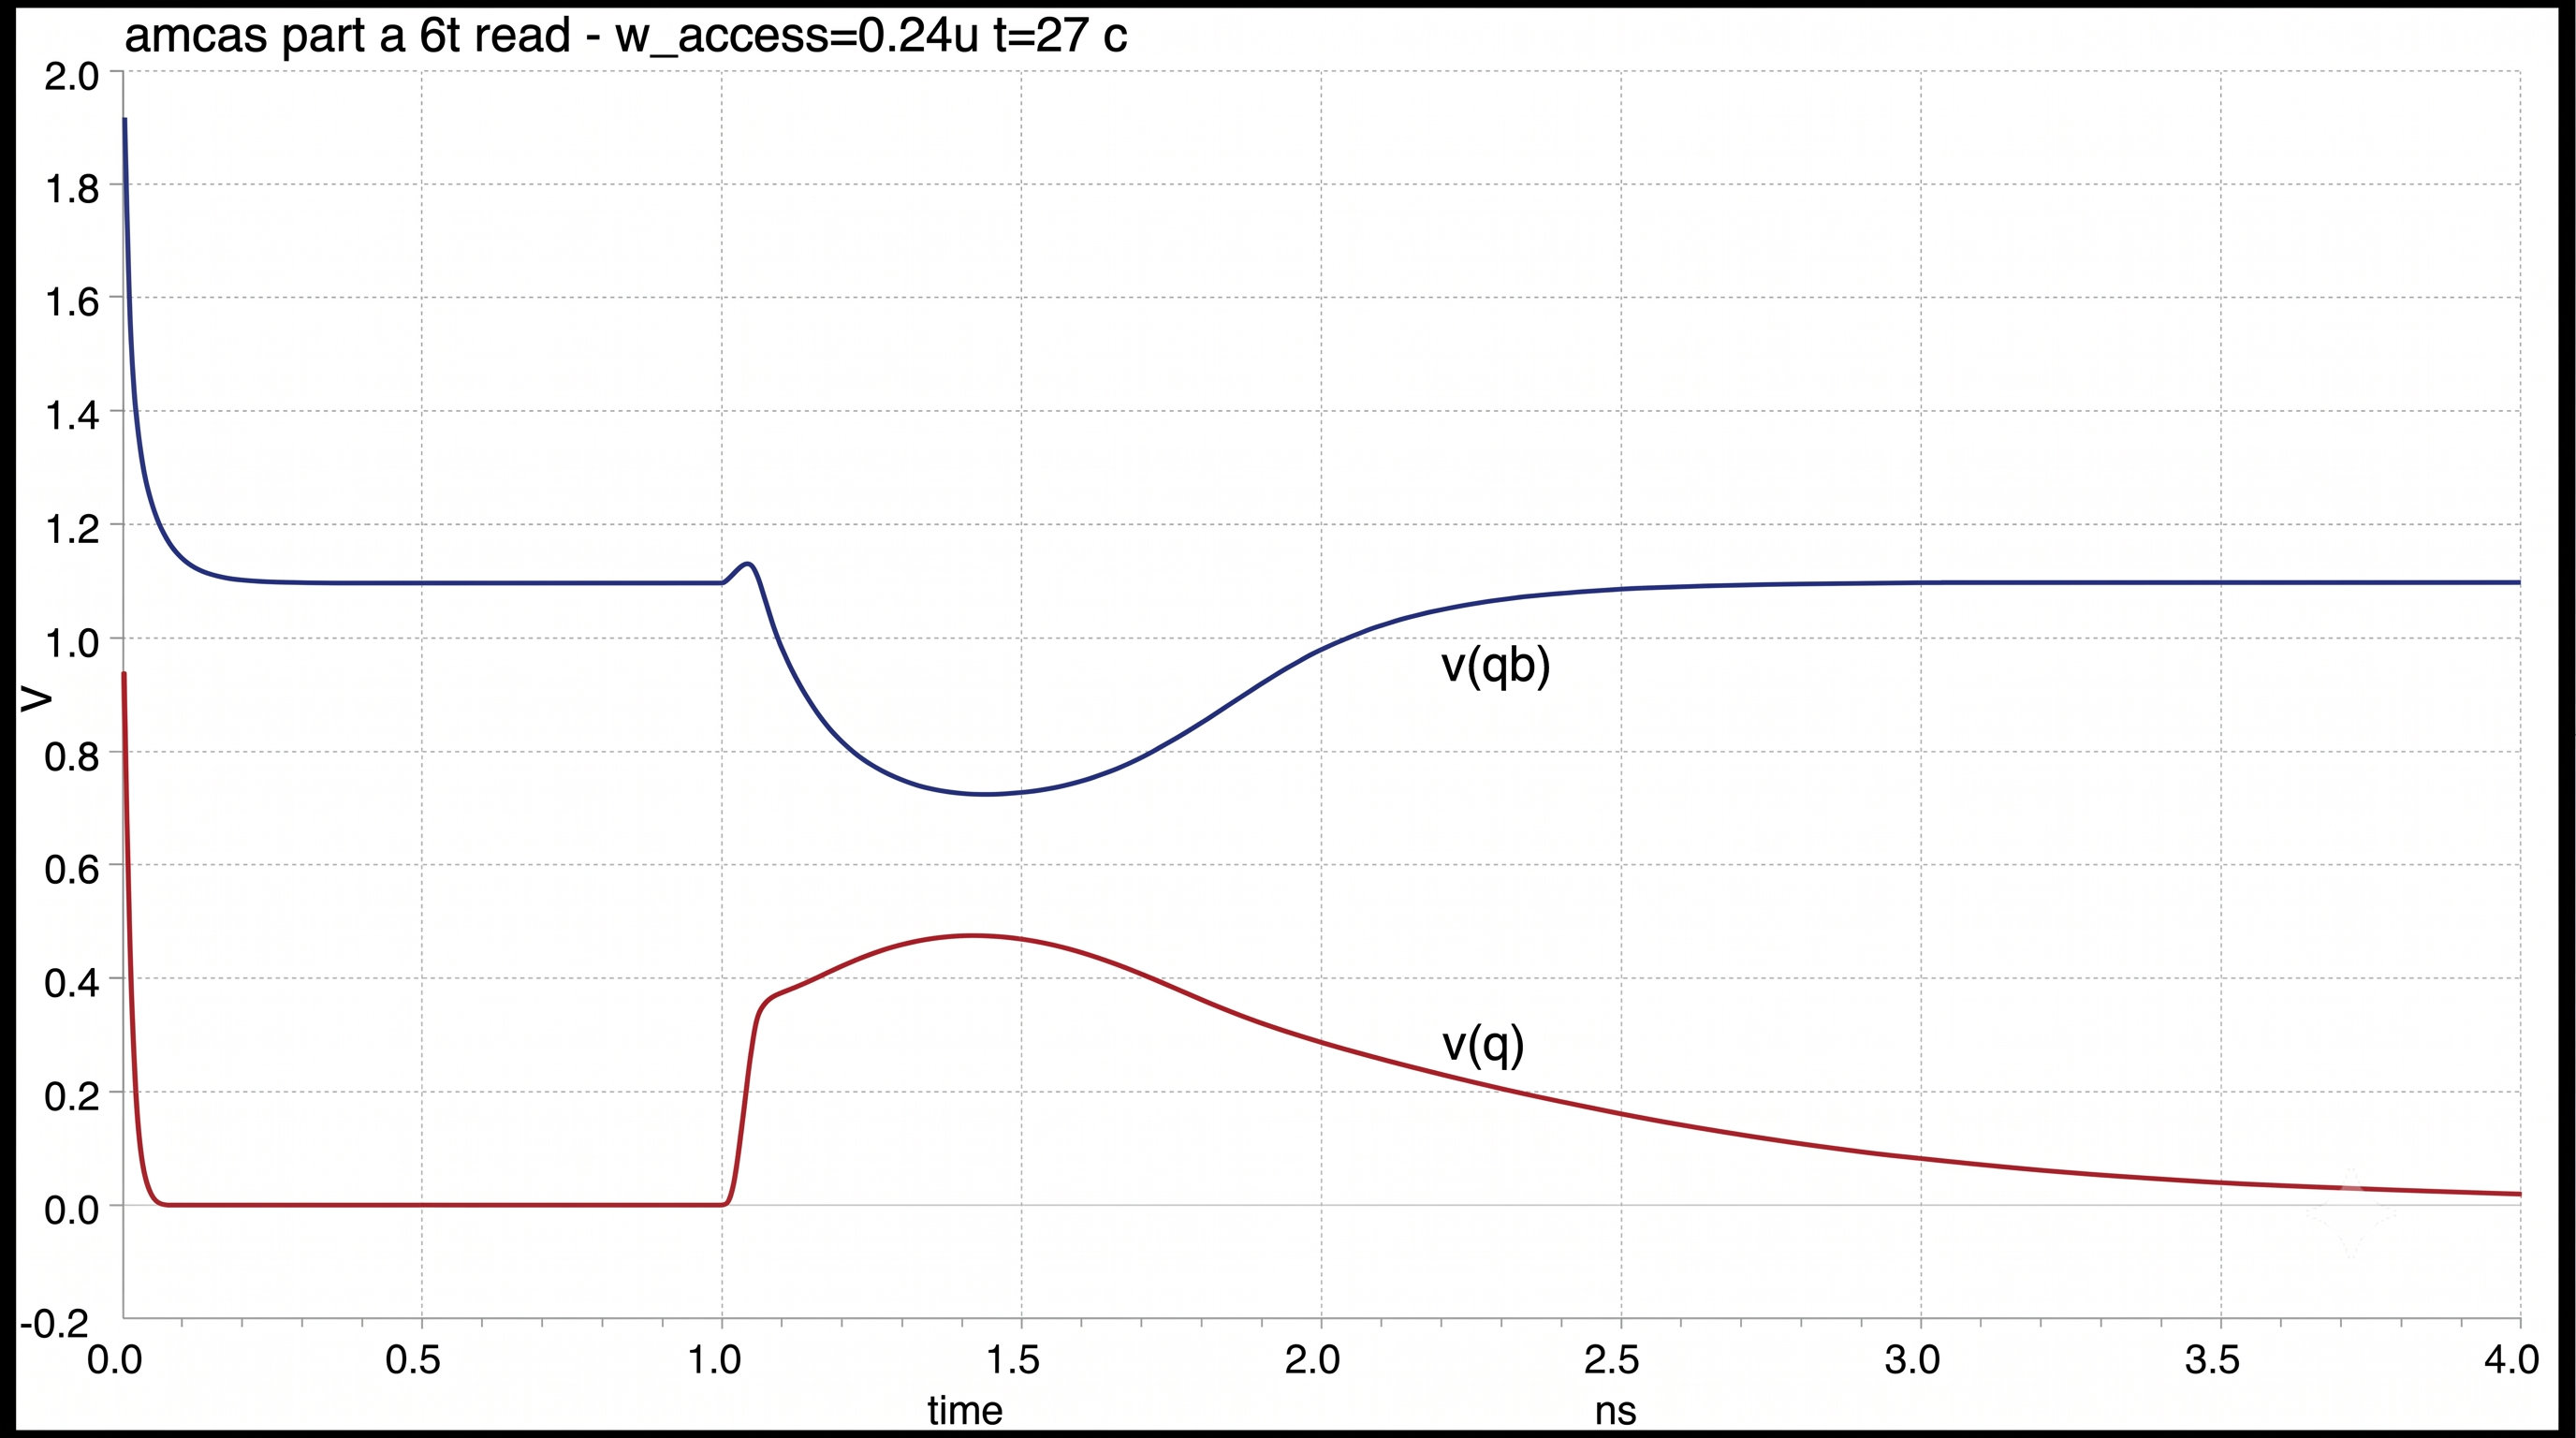
\includegraphics[width=0.5\textwidth]{figures/p1_t2.png}
\caption{$v(Q)$ and $v(\overline{Q})$ at
$W_{acc} = \SI{0.24}{\micro m}$. $Q$ peaks above the trip point shortly
after the wordline rises, then recovers.}
\label{fig:a1}
\end{figure}


\paragraph{Task 3.}

$\Delta V$ falls monotonically with $V_{DD}$ but is still \SI{193}{mV} at
\SI{0.6}{V}, so the \SI{25}{mV} offset is never reached inside the
specified range. Extending the sweep to \SI{0.25}{V} puts the crossing at
\SI{0.32}{V}, barely above the \SI{0.22}{V} threshold voltage and far
below any usable supply.

That result belongs to the measurement instant rather than the device.
Sampling \SI{2}{ns} after the start allows almost a nanosecond of bitline
discharge, roughly ten times a realistic sense amplifier enable delay.
Sampling \SI{100}{ps} after the wordline instead moves the crossing up to
\SI{0.60}{V}, at the bottom of the specified range.

Since the \SI{25}{mV} offset is a mean, \SI{0.32}{V} is only where the
average sense amplifier fails. A design that yields needs more margin than
that, and this netlist cannot say how much because it is symmetric and
carries no device mismatch.

The spike before \SI{0.5}{ns} in the transient plots is a solver artefact,
since \texttt{uic} skips the DC operating point and the simulation starts
unconverged. It settles before the wordline rises and affects no
measurement.

\begin{figure}[!ht]\centering
\includegraphics[width=0.5\textwidth]{figures/p1_t3.png}
\caption{$\Delta V$ against $V_{DD}$, sampled at \SI{2}{ns}, with the
\SI{25}{mV} offset marked. The sweep extends below the specified
\SI{0.6}{V} floor because the offset is not reached within it.}
\label{fig:a2}
\end{figure}

\paragraph{Task 4.}

At \SI{85}{\celsius}, $\Delta V$ barely changes and $q_{max}$ rises by
11\,\%. Neither the read margin nor the sense amplifier offset is what
fails here. Read stability is.

$\Delta V$ stays flat because two effects cancel with temperature, one
helping the read current and one hurting it. The offset does not move
either, since it comes from device mismatch, not temperature.

$q_{max}$ does move. Combined with the wider access devices from Task~2,
this pushes the disturbed node past the trip point, and on a realistic
bitline the read destroys the data.

% \paragraph{Validity.}

% BSIM4 is used, so subthreshold conduction is modelled. Results are
% converged under tight solver tolerances. The netlist is symmetric and
% carries no device mismatch. The measurement statement in the assignment
% fails in ngspice~42 with an unrecognised vector error, so the expression
% is assigned to a vector first.









\section{Part B - CACTI}
\label{sec:b}

Only the parameters the assignment lists were changed from the shipped
\texttt{cache.cfg}. Everything else, including the wire signalling mode
and ECC setting, was left at its default.

\paragraph{How fast, how big, and how leaky is a 2\,MB SRAM L2 at
45\,nm?}

The array takes \SI{2.9018}{ns} to access, occupies \SI{11.474}{mm^2}, and
leaks \SI{2250.5}{mW} across its four banks. These are the numbers every
later part compares against.

\paragraph{Task 1.}

\begin{table}[!ht]\centering\small
\caption{Task 1 baseline. Leakage is reported per bank by CACTI; the
value here is four banks combined.}
\label{tab:b1}
\begin{tabular}{|l|r|}
\hline
Access time & \SI{2.9018}{ns} \\
\hline
Dynamic read energy & \SI{792.9}{pJ} \\
\hline
Leakage & \SI{2250.5}{mW} \\
\hline
Area & \SI{11.474}{mm^2} \\
\hline
\end{tabular}
\end{table}

CACTI's exhaustive search over array organisations selects Ndwl 4, Ndbl 2,
Nspd 1 for the data array.

\paragraph{Task 2.}

Amrutur and Horowitz's claim is one gate delay per doubling of capacity,
which on this axis would be a straight line. That is not what CACTI
produces. The access time increment between adjacent capacities grows
from about 3 gate delays at \SI{256}{kB} to about 86 gate delays at
\SI{16}{MB}, using a \SI{22}{ps} gate delay for 45\,nm. The ratio between
successive points also grows, approaching $\sqrt{2}$ at the largest
sizes, so access time scales with the linear dimension of the array
rather than with the log of its capacity.

\texttt{Ndwl} stays fixed at 4 for the first five capacities in the
sweep. The array is not being resegmented, so each doubling only makes
the existing wordlines and bitlines longer, and wire delay comes to
dominate over the gate delay the claim assumes.

\begin{figure}[!ht]\centering
\includegraphics[width=0.55\textwidth]{figures/p2_t2.png}
\caption{Access time against capacity, with the line one gate delay per
doubling would produce.}
\label{fig:b1}
\end{figure}

\paragraph{Task 3.}

\begin{table}[!ht]\centering\small
\caption{Task 3, three objectives on the same 2\,MB array.}
\label{tab:b2}
\begin{tabular}{|l|c|r|r|}
\hline
Objective & Ndwl / Ndbl & Access time & Area \\
\hline
Delay & 4 / 2 & \SI{2.8923}{ns} & \SI{10.970}{mm^2} \\
\hline
Area & 2 / 2 & \SI{3.3552}{ns} & \SI{9.245}{mm^2} \\
\hline
ED\textsuperscript{2}P & 4 / 2 & \SI{2.9018}{ns} & \SI{11.474}{mm^2} \\
\hline
\end{tabular}
\end{table}

The organisation changes because each objective trades the same thing
differently. More wordline segments shorten each wordline and speed up
the array, but each segment needs its own decoders and sense amplifiers,
which costs area. The delay-optimal and area-optimal runs sit at opposite
ends of that trade, and ED\textsuperscript{2}P lands close to the
delay-optimal point because delay enters the objective squared.

\paragraph{Task 4.}

CACTI reports a bitline delay of \SI{406.9}{ps} for the Task~1 winner.
The hand calculation uses
$t_{50\%} = 0.38\,R_{bl}\,C_{bl}\,L^2$, with each quantity taken from
CACTI's own output or from one stated assumption.

$L$ is the bitline length. CACTI's tech file gives a cell of
\SI{146}{F^2} at an aspect ratio of 1.46, so the cell height is
\SI{0.450}{\micro m}. The winning array has 512 rows per bitline, so
$L = 512 \times \SI{0.450}{\micro m} = \SI{230.4}{\micro m}$.

$C_{bl}$ is taken as \SI{0.35}{fF} per cell, giving
$C_{bl} = 512 \times \SI{0.35}{fF} = \SI{179.2}{fF}$. This matches the
\SI{180}{fF} used for the bitline in Part~A, obtained independently.

$R_{bl}$ is the one assumed quantity. Using a resistivity of
\SI{3.5e-8}{\ohm\metre} over a minimum-width \SI{45}{}$\times$\SI{63}{nm}
cross-section gives \SI{12.3}{\ohm\per\micro m}, so
$R_{bl} = \SI{12.3}{\ohm\per\micro m} \times \SI{230.4}{\micro m}
= \SI{2844}{\ohm}$.

Substituting,
$t_{50\%} = 0.38 \times \SI{2844}{\ohm} \times \SI{179.2}{fF} =
\SI{193.7}{ps}$, against CACTI's \SI{406.9}{ps}, a discrepancy of
\SI{2.1}{\times}.

The gap comes from what the hand formula omits. It models only wire $R$
and $C$, while CACTI's circuit-level model also includes the access
transistor's own resistance in series with the wire, which is the main
source of the discrepancy.






\section{Part C - NVSim}
\label{sec:c}

NVSim's own \texttt{SRAM.cell} is used as the control, run through the
same tool, wire model and search as the STT-MRAM cell. Comparing across
CACTI and NVSim instead would change the tool, the wire model and the
periphery search all at once, which is why that comparison is kept
separate in Sec.~\ref{sec:err}.

\paragraph{Same 2\,MB, same periphery, different bitcell. What changes?}

Leakage and area improve, both latencies get worse, and the two energy
figures stay close. Write latency is the outlier at over twenty times
worse.

\begin{table}[!ht]\centering\small
\caption{Data array results. The upper block compares the two bitcells
under the same tool and configuration. The lower block gives the two
cell-file variations of Tasks~3 and~4.}
\label{tab:c}
\begin{tabular}{|l|r|r|r|}
\hline
Metric & SRAM & STT-MRAM & Ratio \\
\hline
Read latency & \SI{753.4}{ps} & \SI{1.448}{ns} & 1.92$\times$ worse \\
\hline
Write latency & \SI{520.0}{ps} & \SI{10.608}{ns} & 20.4$\times$ worse \\
\hline
Read energy & \SI{561.2}{pJ} & \SI{662.0}{pJ} & 1.18$\times$ worse \\
\hline
Write energy & \SI{517.8}{pJ} & \SI{454.1}{pJ} & 1.14$\times$ better \\
\hline
Leakage & \SI{2.981}{W} & \SI{369.5}{mW} & 8.07$\times$ better \\
\hline
Area & \SI{5.944}{mm^2} & \SI{3.142}{mm^2} & 1.89$\times$ better \\
\hline
\multicolumn{4}{|l|}{\emph{Task 3, doubling TMR}} \\
\hline
& 3\,k/\SI{6}{k\ohm} & 4\,k/\SI{12}{k\ohm} & \\
\hline
Read latency & \SI{1.448}{ns} & \SI{1.453}{ns} & \\
\hline
Sense amplifier latency & \SI{803.455}{ps} & \SI{803.455}{ps} & \\
\hline
\multicolumn{4}{|l|}{\emph{Task 4, halving the reset current}} \\
\hline
& \SI{200}{\micro A} & \SI{100}{\micro A} & \SI{100}{\micro A}, scaled \\
\hline
Area & \SI{3.142}{mm^2} & \SI{3.142}{mm^2} & \SI{2.545}{mm^2} \\
\hline
Array efficiency & 58.4\,\% & 58.4\,\% & 72.1\,\% \\
\hline
\end{tabular}
\end{table}

\paragraph{Task 1.}

The cache-level hit latency including the tag array is \SI{1.589}{ns},
and this is the value carried into Part~E.

\paragraph{Task 2.}

The two that get dramatically worse are read and write latency. Write
latency is the extreme case, and the reason is that the write time is not
a circuit delay at all. The switching pulse alone accounts for \SI{10}{ns}
of the \SI{10.608}{ns} total, so the array spends almost the entire write
waiting for the free layer to flip. Read latency suffers because sensing a
resistance is slower than sensing a charge, and because the denser cell
lets NVSim build a taller subarray, which lengthens the bitline.

The two that get dramatically better are leakage and area. An MRAM cell
holds its state in magnetic orientation and draws nothing to maintain it,
while an SRAM cell is two inverters that conduct continuously. Area
follows from the cell itself, one MTJ stacked above one access transistor
against six transistors laid side by side.

Read energy is the one figure that looks unremarkable and is not. For the
SRAM most of it goes into the H-tree and array overhead, while for the
STT-MRAM most of it is the sense current pushed through the cell. The
totals land close together but almost none of that energy is being spent
on the same thing.

\paragraph{Task 3.}

Nothing moves. Sense amplifier latency is identical to three decimals,
because NVSim sets it from the peripheral circuit rather than from how far
apart the two resistance states sit. Read latency shifts by under one
percent and in the wrong direction, since reaching the higher ratio meant
raising $R_{on}$, which slows the read current.

So a TMR headline buys separation between the two states in principle. At
the array level it only pays off if the sense circuit is designed to
exploit that separation, and in this model it is not.

\paragraph{Task 4.}

Halving the current on its own does nothing to the area. The shipped cell
file states the cell area and the access transistor width as fixed
numbers instead of deriving them from the write current, so the two are
simply not connected in that run.

Allowing the transistor to shrink with the current recovers the effect.
Area drops and array efficiency rises sharply, because the write current
is what forces the access transistor to be wide, the transistor is what
sets the cell pitch, and the cell pitch is what determines how much of the
density advantage actually reaches the array. That chain is the reason
write current matters so much in NVM design, and it stays invisible here
only because the cell file pins two of its links.








\section{Part D - DRAMsim3}
\label{sec:d}

The trace is the L2 miss stream captured from the Part~E baseline run,
using a \texttt{CommMonitor} on the L2 memory-side port. Of the packets
captured, \SI{35.9}{\percent} were \texttt{CleanEvict} notifications that
carry no data and never reach DRAM, so those are dropped. The remaining
500\,000 requests are \SI{81.3}{\percent} reads and \SI{18.7}{\percent}
writes, spread over 37.3\,million memory cycles. The default cycle budget
completes only a small fraction of that, so the runs use 40\,million
cycles to let the whole stream finish.

\paragraph{Does the changed miss traffic still fit in one DDR4 channel?}

Comfortably. The requests arrive on average 74.6 cycles apart, which
leaves the channel close to idle, and a second channel improves latency by
under ten percent.

\begin{table}[!ht]\centering\small
\caption{All four configurations in DRAMsim3, with Ramulator 2.1 shown
for the two tasks it can run. Baseline is open row, one channel, row bits
above bank bits. Latency in memory cycles.}
\label{tab:d}
\begin{tabular}{|l|r|r|r|r|}
\hline
& \multicolumn{2}{c|}{DRAMsim3} & \multicolumn{2}{c|}{Ramulator 2.1} \\
\hline
Configuration & Hit rate & Read latency & Hit rate & Read latency \\
\hline
Baseline (Task 1) & 84.73\,\% & 53.53 & 99.93\,\% & 270.90 \\
\hline
Closed row (Task 2) & 0.00\,\% & 582.16 & 49.94\,\% & 1224.16 \\
\hline
Row below bank (Task 3) & 50.33\,\% & 142.32 & \multicolumn{2}{c|}{not expressible} \\
\hline
Two channels (Task 4) & 88.56\,\% & 48.21 & \multicolumn{2}{c|}{not expressible} \\
\hline
\end{tabular}
\end{table}

\paragraph{Task 1.}

The baseline completes all 406\,608 reads and 93\,393 writes at a
row buffer hit rate of \SI{84.73}{\percent} and an average read latency of
53.53 cycles.

\paragraph{Task 2.}

Neither simulator offers an FCFS scheduler, so a closed row policy is used
instead. It removes row reuse between accesses, which is the effect the
task asks about.

The latency rises by 528 cycles, far more than the 44 cycles that
$t_{RCD} + t_{RP}$ would suggest. That figure is the cost of one isolated
row miss. What the simulation reports is the queueing that follows once
every access needs its own activate and precharge. Because those accesses
target the same bank, they serialise at $t_{RC}$, which is 74 cycles each,
and per-bank throughput collapses. The latency is dominated by the queue
that builds up, not by the activate and precharge pair itself.

\paragraph{Task 3.}

Latency rises by a factor of 2.66 while the row buffer hit rate only falls
to half, so this is not mainly a loss of row locality. It is a loss of
bank level parallelism. With the row bits below the bank bits, addresses
that used to spread across sixteen banks now land in the same one, and
requests queue behind a single bank's row cycles instead of overlapping
across many.

\paragraph{Task 4.}

Latency improves by under ten percent, so bandwidth was never the limit.
The trace delivers a request every 74.6 cycles on average, and a
DDR4-3200 channel can retire one every few cycles, so the channel is only
lightly loaded to begin with. A second channel has almost nothing to take
over.

The binding constraint is $t_{RC}$, at 74 cycles the time a bank needs
between successive row activations. The arrival interval and $t_{RC}$ are
nearly equal, so the array is limited by how fast a single bank can cycle
rather than by how fast the channel can carry data. The small gain that
does appear comes from each channel seeing slightly better row locality
once the stream is split, which is why the hit rate rises while the
latency barely moves.

\paragraph{Cross check against Ramulator.}

The two simulators disagree by a factor of five on baseline read latency.
The main reason is the trace format. Ramulator's reader has no arrival
time field, so it issues requests as fast as the queue accepts them and
runs the channel saturated, while DRAMsim3 replays the spacing gem5
actually produced. The row hit rates also differ because the closed row
substitutions are not the same, one allowing a single hit per activation
and the other precharging after every access. Sec.~\ref{sec:err} returns
to this.









\section{Part E - gem5}
\label{sec:e}

Two GAPBS kernels are run on three L2 configurations. The hit latencies
come from Parts~B and~C, and the capacity from NVSim's areas. The
handout's own assumption of \SI{8}{MB} at 14 cycles is also run, since it
matches neither measurement.

\texttt{-{}-l2-hit-latency} is not a valid \texttt{se.py} option, so the
latency is set in \texttt{configs/common/Caches.py}. The graphs are built
outside the simulation, because generating them inside leaves the
traversal at under one percent of the program and the measured window
lands entirely in graph construction.

\paragraph{Does the program actually run faster?}

On bfs yes, by \SI{1.369}{\times}. On sssp no, by \SI{1.007}{\times},
which is no change at all.
\begin{table}[!ht]\centering\small
\caption{All nine runs. The SRAM rows are the CACTI baseline. The two MRAM
rows differ only in where their numbers came from, one from our own NVSim
measurement and one from the assumption the handout states.}
\label{tab:e}
\begin{tabular}{|l|l|l|l|l|r|r|r|}
\hline
Cell & Source & L2 & Latency & CPU & simSeconds & IPC & Miss rate \\
\hline
\multicolumn{8}{|l|}{\emph{bfs}} \\
\hline
SRAM & CACTI & \SI{2}{MB} & 6 & O3 & 0.081057 & 0.5768 & 0.6403 \\
\hline
MRAM & NVSim & \SI{4}{MB} & 4 & O3 & 0.068778 & 0.6798 & 0.4589 \\
\hline
MRAM & handout & \SI{8}{MB} & 14 & O3 & 0.059203 & 0.7897 & 0.2039 \\
\hline
\multicolumn{8}{|l|}{\emph{sssp}} \\
\hline
SRAM & CACTI & \SI{2}{MB} & 6 & O3 & 0.306604 & 0.5967 & 0.1763 \\
\hline
MRAM & NVSim & \SI{4}{MB} & 4 & O3 & 0.261801 & 0.6988 & 0.1435 \\
\hline
MRAM & handout & \SI{8}{MB} & 14 & O3 & 0.304559 & 0.6007 & 0.1276 \\
\hline
\multicolumn{8}{|l|}{\emph{bfs on TimingSimple, for Task 3}} \\
\hline
SRAM & CACTI & \SI{2}{MB} & 6 & TS & 0.250807 & 0.1864 & 0.6432 \\
\hline
MRAM & NVSim & \SI{4}{MB} & 4 & TS & 0.216890 & 0.2156 & 0.4260 \\
\hline
MRAM & handout & \SI{8}{MB} & 14 & TS & 0.196929 & 0.2374 & 0.1779 \\
\hline
\end{tabular}
\end{table}

\paragraph{Task 1.}

The six O3 runs give the baseline and both alternatives for each kernel.
Under our own device numbers, \SI{4}{MB} at 4 cycles, bfs gains
\SI{1.179}{\times} and sssp \SI{1.171}{\times}. Under the handout's
\SI{8}{MB} at 14 cycles, bfs gains \SI{1.369}{\times} and sssp
\SI{1.007}{\times}.

\paragraph{Task 2.}

The trade wins on bfs and does nothing on sssp, and the property that
decides it is the baseline hit rate rather than the size of the working
set. This is not the obvious answer, since sssp has the larger working set
of the two and benefits less.

At \SI{2}{MB}, bfs misses on \SI{64}{\percent} of its 2.56\,million L2
accesses and has only 0.92\,million hits. sssp misses on
\SI{17.6}{\percent} of 28.8\,million accesses and has 23.7\,million hits.
Quadrupling the capacity converts a similar number of misses in both
cases, roughly 1.1 and 1.4\,million, but the eight extra cycles per hit
land on 2.0\,million hits for bfs against 25.1\,million for sssp. The hit
cost rises from 5.5 to 28.3\,million cycles for bfs, and from 142 to
352\,million for sssp, which is enough to cancel everything the extra
capacity gained.

Extra capacity pays off when the baseline cache is already failing. When
it is working, the latency is charged on every hit while very few misses
are recovered.

Under our own measured numbers the trade disappears. The MRAM
configuration is both larger and faster per hit, so both kernels improve
by about seventeen percent and there is nothing to weigh against anything.


\begin{figure}[!ht]\centering
\includegraphics[width=0.55\textwidth]{figures/p5_t2.png}
\caption{Speedup over the \SI{2}{MB} SRAM baseline on an O3 core. Under
the handout's parameters the two kernels diverge. Under our measured
parameters they do not. The shaded band is the compounded error of
Sec.~\ref{sec:err}, and sssp's result lies entirely inside it.}
\label{fig:e}
\end{figure}



\paragraph{Task 3.}

Moving the winning configuration to \texttt{TimingSimple} shrinks the
advantage from \SI{1.369}{\times} to \SI{1.274}{\times}. The reason shows
in which configuration loses more by going in order. The \SI{2}{MB} run
slows by \SI{3.094}{\times} and the \SI{8}{MB} run by
\SI{3.326}{\times}.

The larger cache degrades more because it has 2.02\,million hits at 14
cycles against 0.92\,million at 6. On an out of order core those long hits
overlap with independent instructions and other memory operations in
flight, so most of the latency never reaches the critical path.
\texttt{TimingSimple} issues one instruction at a time and blocks on every
access, so the extra cycles per hit are fully exposed.

Out of order execution was hiding the MRAM configuration's latency
penalty, which means the Task~1 result flatters that cache. The penalty
was always there and O3 was paying it out of slack. On a core with less
tolerance for latency, which an accelerator may well be, the trade looks
worse.





\section{Error budget}
\label{sec:err}

The assignment quotes ngspice at \SI{5}{\percent}, CACTI and Ramulator at
\SI{10}{\percent}, and gem5 at \SI{20}{\percent}, compounding
multiplicatively. Part~E's results pass through CACTI for latency, NVSim
for area and gem5 for cycles, which compounds to \SI{24.5}{\percent} in
quadrature.

\begin{table}[!ht]\centering\small
\caption{Every reported ratio against the compounded band.}
\label{tab:err}
\begin{tabular}{|l|r|l|c|}
\hline
Result & Value & Range & Distinguishable from 1.0 \\
\hline
Part C write latency & 20.40$\times$ & 15.4 to 25.4 & yes \\
\hline
Part D closed row & 10.90$\times$ & 8.2 to 13.6 & yes \\
\hline
Part C leakage & 8.07$\times$ & 6.1 to 10.1 & yes \\
\hline
Part D row below bank & 2.66$\times$ & 2.0 to 3.3 & yes \\
\hline
Part B bitline hand check & 2.10$\times$ & 1.6 to 2.6 & yes \\
\hline
Part C area & 1.89$\times$ & 1.4 to 2.4 & yes \\
\hline
Part E bfs speedup & 1.369$\times$ & 1.03 to 1.70 & marginally \\
\hline
Part E sssp speedup & 1.007$\times$ & 0.76 to 1.25 & no \\
\hline
Part C TMR effect & 1.004$\times$ & 0.76 to 1.25 & no \\
\hline
Part D two channels & 0.90$\times$ & 0.68 to 1.12 & no \\
\hline
\end{tabular}
\end{table}

The three results that fall inside the band are the three null results,
which is the right way to report them. Doubling TMR moved nothing, sssp
gained nothing, and a second channel gained nothing, and in each case the
change cannot be resolved under the assignment's own budget. The headline
is therefore \SI{1.369}{\times} on bfs, with a range of 1.03 to 1.70.

\paragraph{The stated budget is optimistic.}

Given the same \SI{2}{MB} SRAM with the same cell, CACTI and NVSim
disagree by \SI{3.41}{\times} on access time and \SI{1.79}{\times} on
area. Given the same trace, Ramulator and DRAMsim3 disagree by
\SI{5.06}{\times} on read latency. Against a stated \SI{10}{\percent}
these are 8 to 41 times too large.

The published error bars describe each tool measured against silicon it
was validated on. This chain is tool to tool, on configurations none of
them was validated for, so the uncertainty that governs the result is how
far the tools disagree with each other rather than how far each sits from
hardware. That difference is not academic. It is the reason the central
question changes character depending on whether the MRAM hit latency comes
from NVSim, at 4 cycles and faster than the SRAM, or from the handout's
assumption, at 14 cycles and slower.







\section{Part E Task 4 - the argument}

\paragraph{Should the 2\,MB L2 be SRAM or STT-MRAM?}

Conditionally STT-MRAM. Part~C measured \SI{8.07}{\times} lower leakage
and \SI{1.89}{\times} less area, and at iso-area Part~E showed that buys
\SI{1.369}{\times} on bfs. Part~D confirmed the channel is only ten
percent utilised either way, so nothing downstream objects.

The win needs three conditions together.

\begin{itemize}
\item A workload whose cache is already failing. bfs at \SI{64}{\percent}
misses gained; sssp at \SI{17.6}{\percent} gained nothing.
\item A core that tolerates latency. Task~3 showed out of order execution
was concealing seven points of the advantage.
\item A read-dominated access pattern. Neither kernel writes enough to
expose the \SI{20.4}{\times} write penalty, so a write-heavy workload
would likely reverse the verdict.
\end{itemize}

MRAM's strongest result also never reaches the Part~E answer, since gem5
reports cycles and not joules. On a power-limited accelerator that
probably matters more than the \SI{1.369}{\times}.

\paragraph{Assumptions I would attack as a reviewer.}

\begin{itemize}
\item \textbf{The tools disagree with each other more than with silicon.}
CACTI and NVSim differ by \SI{3.41}{\times} on the same SRAM, Ramulator
and DRAMsim3 by \SI{5.06}{\times} on the same trace, against published
bars of \SI{10}{\percent}. This is why the MRAM cache appears faster per
hit, which removes the trade entirely.

\item \textbf{The cell file states its own answer.} Halving the write
current moved the area not at all until the transistor width was allowed
to scale. Every area-derived number inherits this, including Part~E's
iso-area capacity.

\item \textbf{Nothing carries any variation.} No $\sigma$, no yield,
sixteen million identical cells. Part~A's \SI{0.32}{V} crossing is where
the average sense amplifier fails, not a usable supply, and a self-heating
array is invisible even though MRAM switching current depends on
temperature.

\item \textbf{The trace cannot react.} Part~D replays arrival times gem5
fixed before the DRAM configuration was changed. A slower memory never
delays the next request, so the latency answers in Tasks~2 and~4 describe
a machine that is not allowed to respond to them.

\end{itemize}






\section*{Reproducibility}
\small
All configurations, scripts and results:
\url{https://github.com/Jayadeep-4/AMCAS-assignment1}. Each part has a
README with the clone URL, build command and any patch required. Two tools
need source changes: NVSim requires \texttt{-std=c++11}, and gem5 requires
the L2 latency to be set in \texttt{Caches.py} because no command-line
option exists.


\end{document}